\documentclass{beamer}[10pt, usepdftitle=false, handout]

\beamertemplatenavigationsymbolsempty

\usepackage[T1]{fontenc}
\usepackage[]{algorithm2e}
\usepackage{multimedia}
\usepackage{gensymb}
\usepackage{textcomp}
%\usepackage{background}
%\backgroundsetup{
%    placement=center,
%    scale=1,
%    contents={The author of this course is PAUL BLONDEL},
%    opacity=0.7
%}
%\setbeamertemplate{background}{\BgMaterial}

%\usepackage[font=small,labelfont=bf]{caption} 

\usetheme{Boadilla}

\title{Operating system principles 3}
\author[]{Paul Blondel}
\institute[]{CNAM}
\date[]{September 1st, 2018}

\usepackage[style=british]{csquotes}


\def\signed #1{{\leavevmode\unskip\nobreak\hfil\penalty50\hskip1em
  \hbox{}\nobreak\hfill #1%
  \parfillskip=0pt \finalhyphendemerits=0 \endgraf}}

\newsavebox\mybox
\newenvironment{aquote}[1]
  {\savebox\mybox{#1}\begin{quote}\openautoquote\hspace*{-.7ex}}
  {\unskip\closeautoquote\vspace*{1mm}\signed{\usebox\mybox}\end{quote}}


%\setbeamertemplate{headline}
%{
%  \leavevmode%
%  \hbox{%
%  \begin{beamercolorbox}[wd=1.0\paperwidth,ht=2.25ex,dp=1ex,center]{author in head/foot}%
%   \textcolor{green}{- This course has been made by Paul Blondel -} \usebeamerfont{author in head/foot}\insertsubsection
%  \end{beamercolorbox}}%
%  \vskip0pt%
%}


\setbeamertemplate{footline}
{
  \leavevmode%
  \hbox{%
  \begin{beamercolorbox}[wd=.5\paperwidth,ht=2.25ex,dp=1ex,center]{author in head/foot}%
    \usebeamerfont{author in head/foot}\insertsection
  \end{beamercolorbox}%
  \begin{beamercolorbox}[wd=.5\paperwidth,ht=2.25ex,dp=1ex,center]{title in head/foot}%
    \usebeamerfont{title in head/foot} \inserttitle \hspace*{2em}  \insertframenumber{} / \inserttotalframenumber\hspace*{2ex} 
  \end{beamercolorbox}}%
  \vskip0pt%
}

\AtBeginSection[]
{
   \begin{frame}
    \tableofcontents[ 
    currentsection,
    hideallsubsections] 
   \end{frame}
}

\begin{document}
	{
	\setbeamertemplate{footline}{
  	\leavevmode%
  	\hbox{%
  	\begin{beamercolorbox}[wd=.5\paperwidth,ht=2.25ex,dp=1ex,center]{author in head/foot}%
  	\end{beamercolorbox}%
  	\begin{beamercolorbox}[wd=.5\paperwidth,ht=2.25ex,dp=1ex,center]{title in head/foot}%
  	\end{beamercolorbox}}%
  	\vskip0pt%	
	} 
	\begin{frame}
	\titlepage
	\end{frame}

	\begin{frame}
	
	\begin{aquote}{Eric S. Raymond}
	(Kenneth) Thompson and (Dennis) Ritchie were among the first to realize that hardware and compiler technology had become good enough that an entire operating system could be written in C, and by 1978 the whole environment had been successfully ported to several machines of different types.	
	\end{aquote}	
	
	\end{frame}

	\begin{frame}
		\tableofcontents[hideallsubsections]
	\end{frame}
	}

	\addtocounter{framenumber}{-3}

	\section{Introduction}

    \begin{frame}[label=(first)]
	
	\begin{block}{Recall}
	The \textit{main memory} is where \textit{running software} and \textit{opened documents} are.
	
	It's \textbf{important to well manage the main memory}:
	\begin{itemize}
	\item{The \textbf{more software we launch, the more data} we use}
	\item{If \textbf{not enough memory: cannot execute new softwares}}
	\end{itemize}	 
	\end{block}
	
	\vspace*{1em}
	
	In the \textit{main memory} for each process:
	\vspace*{1em}
	\begin{itemize}
	\item{there is a \textit{starting} and an \textit{ending address}}	
	\item{there is an associated \textit{allocated data}}
	\item{the allocated data is \textit{protected from other processes}}
	\end{itemize}		
	
    \end{frame}
    
	\subsection{Definitions}
	
	\begin{frame}
	\begin{exampleblock}{Virtual memory}	
	The \textit{virtual memory} \textbf{is stored in the \textit{mass storage memory}} and is \textbf{used when the \textit{main memory} is filled}
	\end{exampleblock}	
	
	\begin{exampleblock}{Physical memory}
	The  \textit{physical memory} is \textbf{stored in the \textit{main memory}}, you cannot have more physical memory than the main memory. \footnotemark[1]
	\end{exampleblock}

	\begin{exampleblock}{Logic addresses}
	These are the \textbf{addresses within the executable when it is in the \textit{mass storage memory}} (before getting loaded in the main memory)
	\end{exampleblock}
	
	\begin{exampleblock}{Physical addresses}
	These are the \textbf{addresses within the executable when it is loaded in \textit{main memory}}
	\end{exampleblock}	
	
	\footnotemark[1]{The physical memory space is where software and opened documents are.}	
	
	\end{frame}	
	
	\subsection{Allocating in the physical memory space}	
		    
	\begin{frame}
	When a user launches an \textit{executable}:	
	\vspace*{0.5em}
	\begin{itemize}
	\item{The \textbf{loader loads the executable in main memory}
		\begin{itemize}
		\item{The loader \textbf{must find a place big enough} in main memory}
		\item{Memory is allocated at this location}
		\item{\textit{logical addresses} are \textbf{converted} into \textit{physical addresses}}
		\end{itemize}
	}
	\end{itemize}
	
	\pause	
	
	\vspace*{0.5em}	
	
	When the \textit{process} has terminated its execution:
	\vspace*{0.5em}
	\begin{itemize}
	\item{The \textit{allocated memory} is \textbf{freed from the memory}}
	\item{This memory is \textbf{available again} for other \textit{processes}}
	\end{itemize}			
		
	\vspace*{0.5em}		
		
	\begin{block}{Two approaches}
	There are \textit{two approaches} to \textbf{allocate} and \textbf{release memory}:
	\begin{enumerate}
	\item{\textbf{Contiguous approach}: one program = one \textbf{unique} and \textbf{inseparable} memory \textbf{partition}}
	\item{\textbf{Non-contiguous approach}:  one program = set of \textbf{separable parts dispatched in memory}}
	\end{enumerate}	
	\end{block}
		
	\end{frame}	    
	    	
	\section{Contiguous allocation of the physical memory}	    	
	\subsection{Principle}
	    	
	\begin{frame}
	\begin{block}{Contiguous?}
	Here an executable is loaded in \textbf{one inseparable block of data} in memory
	\end{block}
	
	\vspace*{1em}
	Here ...
	\vspace*{0.5em}
	\begin{itemize}
	\item{The \textit{loader} looks for the \textbf{best free area in memory} to load}
	\item{Once the \textit{process} is terminated the \textbf{block of data is freed}}
	\end{itemize}	
	
	\begin{figure}
		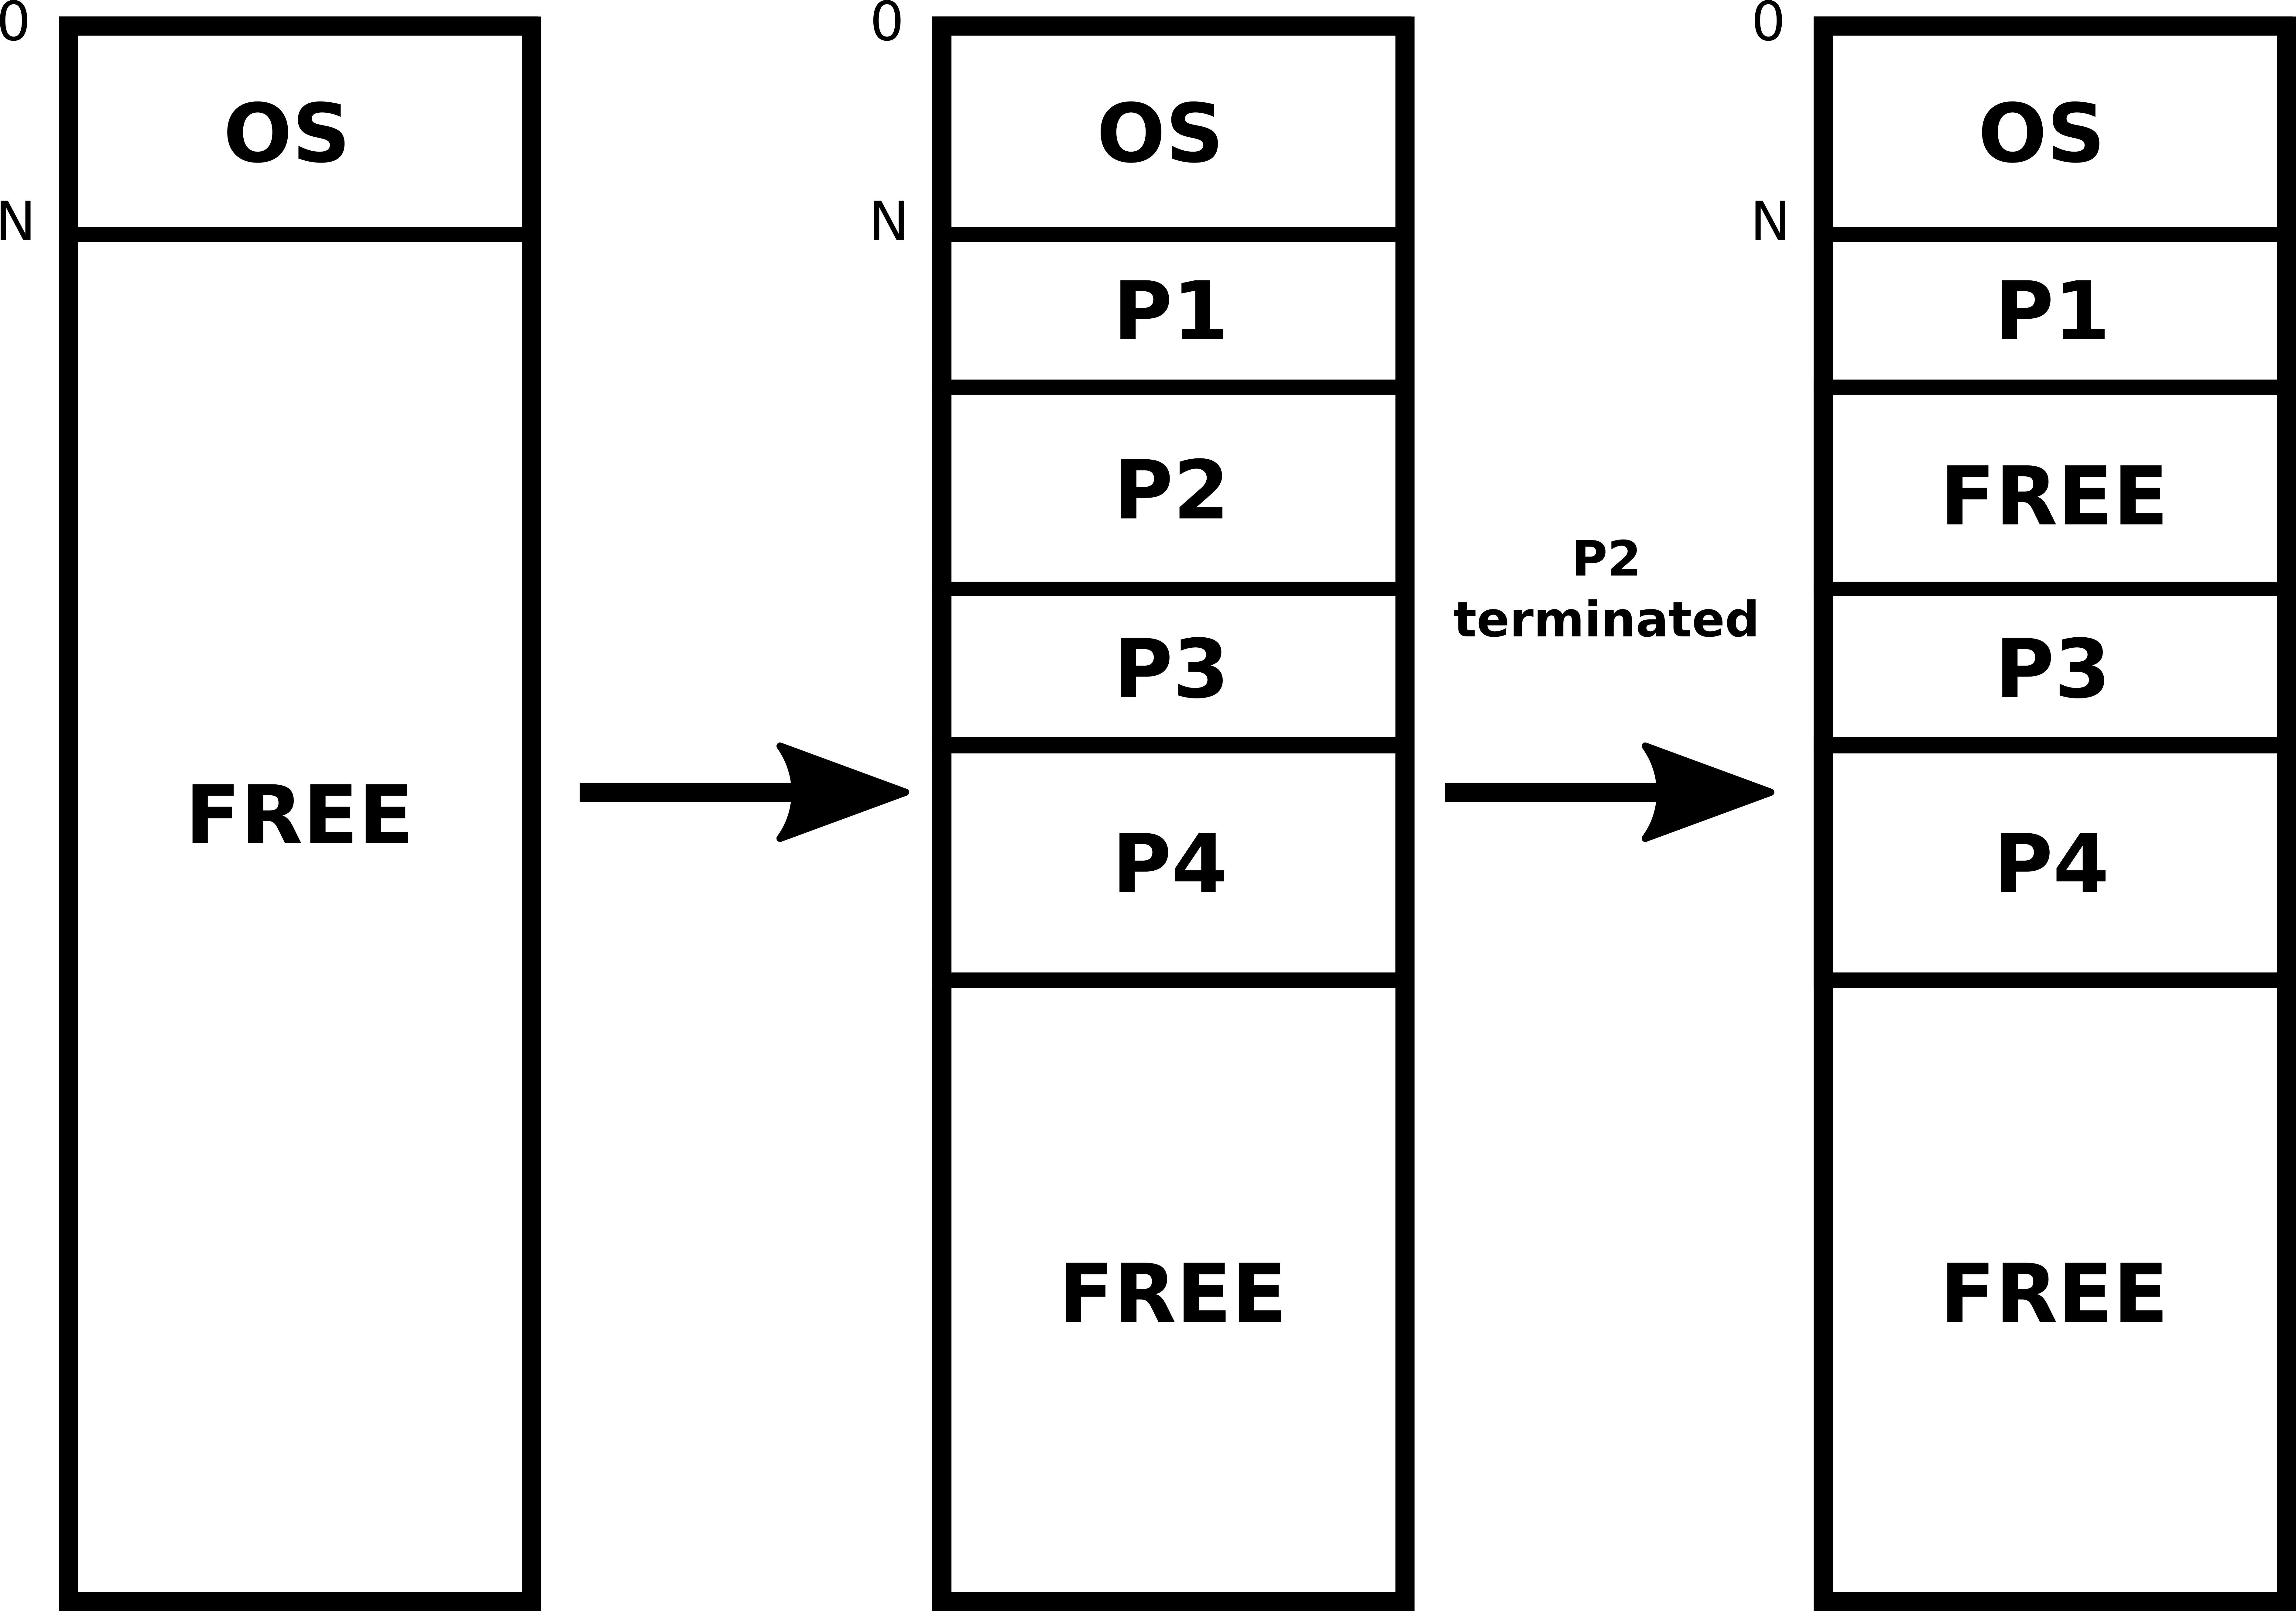
\includegraphics[scale=0.05]{images/p_mem_1.png} 
     	%\vspace*{-0.5em}
		%\caption{Floating gate transistor cell}
	\end{figure}	
	
	
	\end{frame}
	   
	\subsection{Allocating methods of the free memory}
	\begin{frame}

	Loading a new program in memory consists in ...
	\vspace*{1em}
	\begin{itemize}
	\item{... finding a \textbf{big enough free area} to load the the program}
	\item{... \textbf{minimizing the wasted space} in main memory}
	\item{... \textbf{minimizing the time spent} to find the best place}
	\end{itemize}		
	
	\pause
	\vspace*{1em}
	\textbf{Three strategies} to find a contiguous free area:
	\vspace*{0.5em} 
	\begin{enumerate}
	\item{The "\textit{First free area}" strategy}
	\item{The "\textit{Best free area}" strategy}
	\item{The "\textit{Worst free area}" strategy}
	\end{enumerate}
	
	\end{frame}   
	    	
	\begin{frame}
	The "\textit{First free area}" strategy:
	\vspace*{1em}	
		
	\begin{figure}
		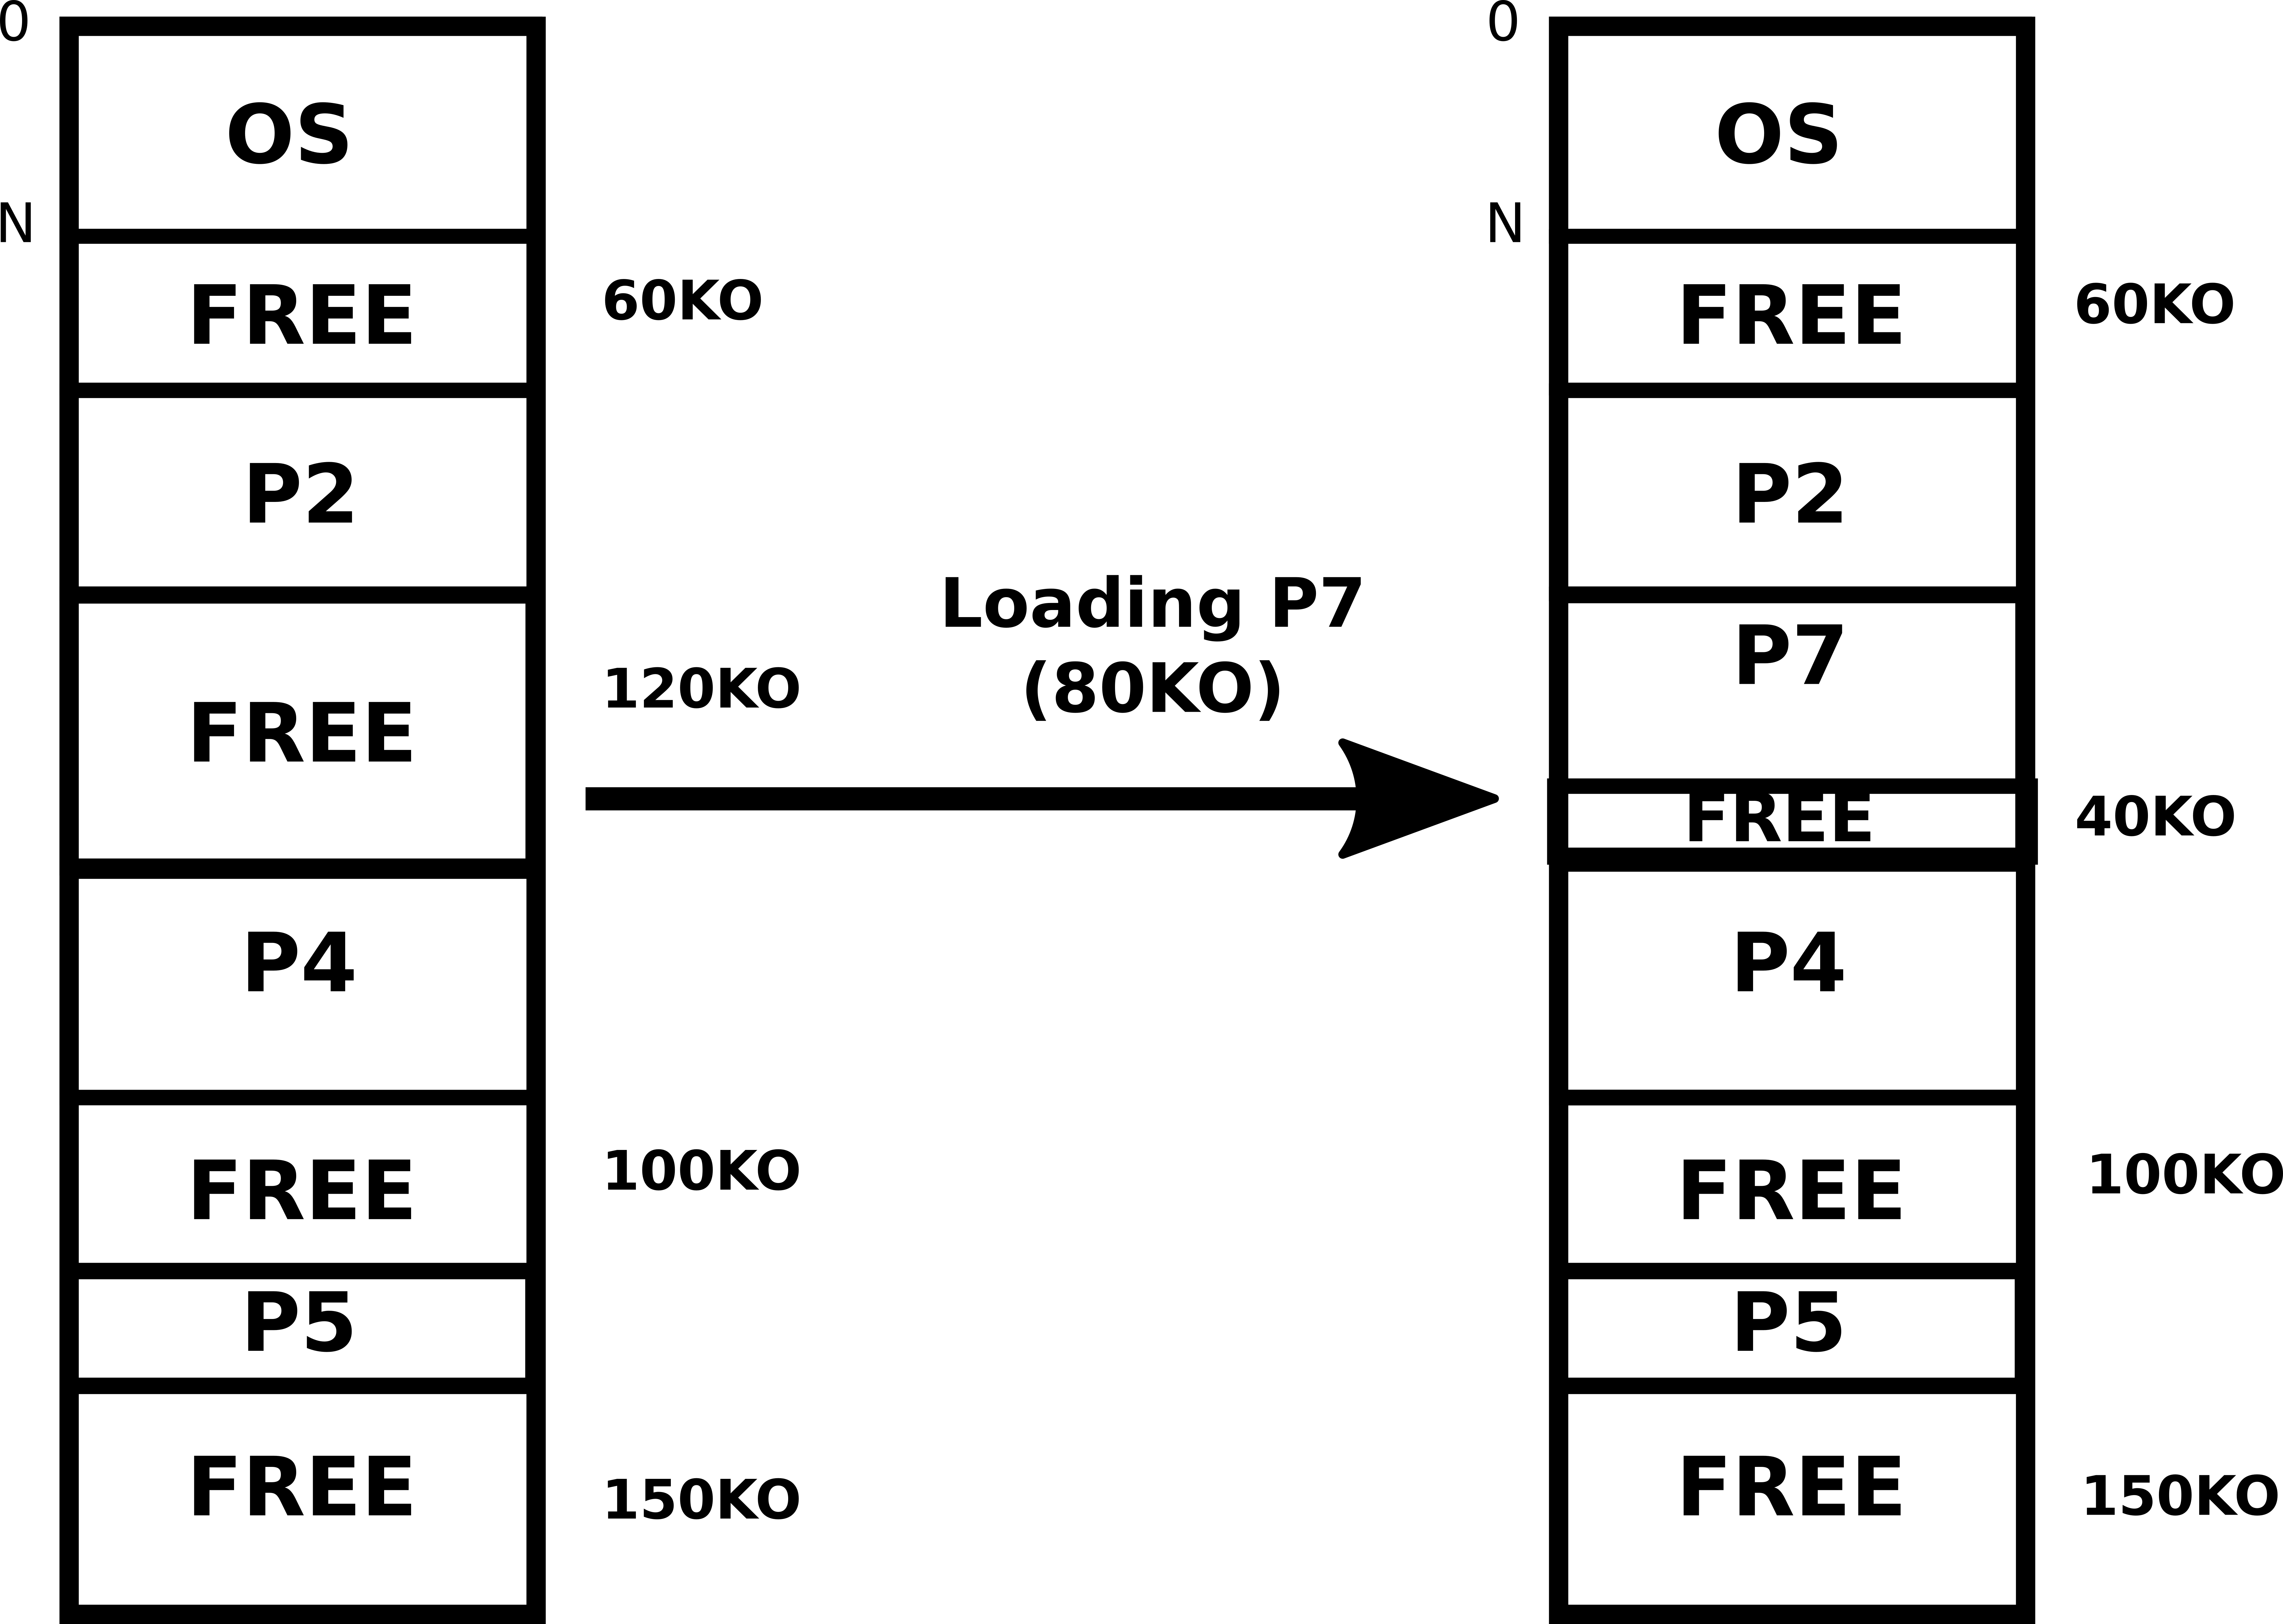
\includegraphics[scale=0.05]{images/p_mem_2.png} 
     	%\vspace*{-0.5em}
		%\caption{Floating gate transistor cell}
	\end{figure}	
	
	\vspace*{1em}
	\begin{itemize}
	\item{Advantage: \textbf{Fastest approach}}
	\item{BUT: \textbf{Not designed to optimize the main memory usage} (40KO)}
	\end{itemize}		
	
	
	\end{frame}	    	
	    	
	\begin{frame}
	
	The "\textit{Best free area}" strategy:
	\vspace*{1em}
	
	\begin{figure}
		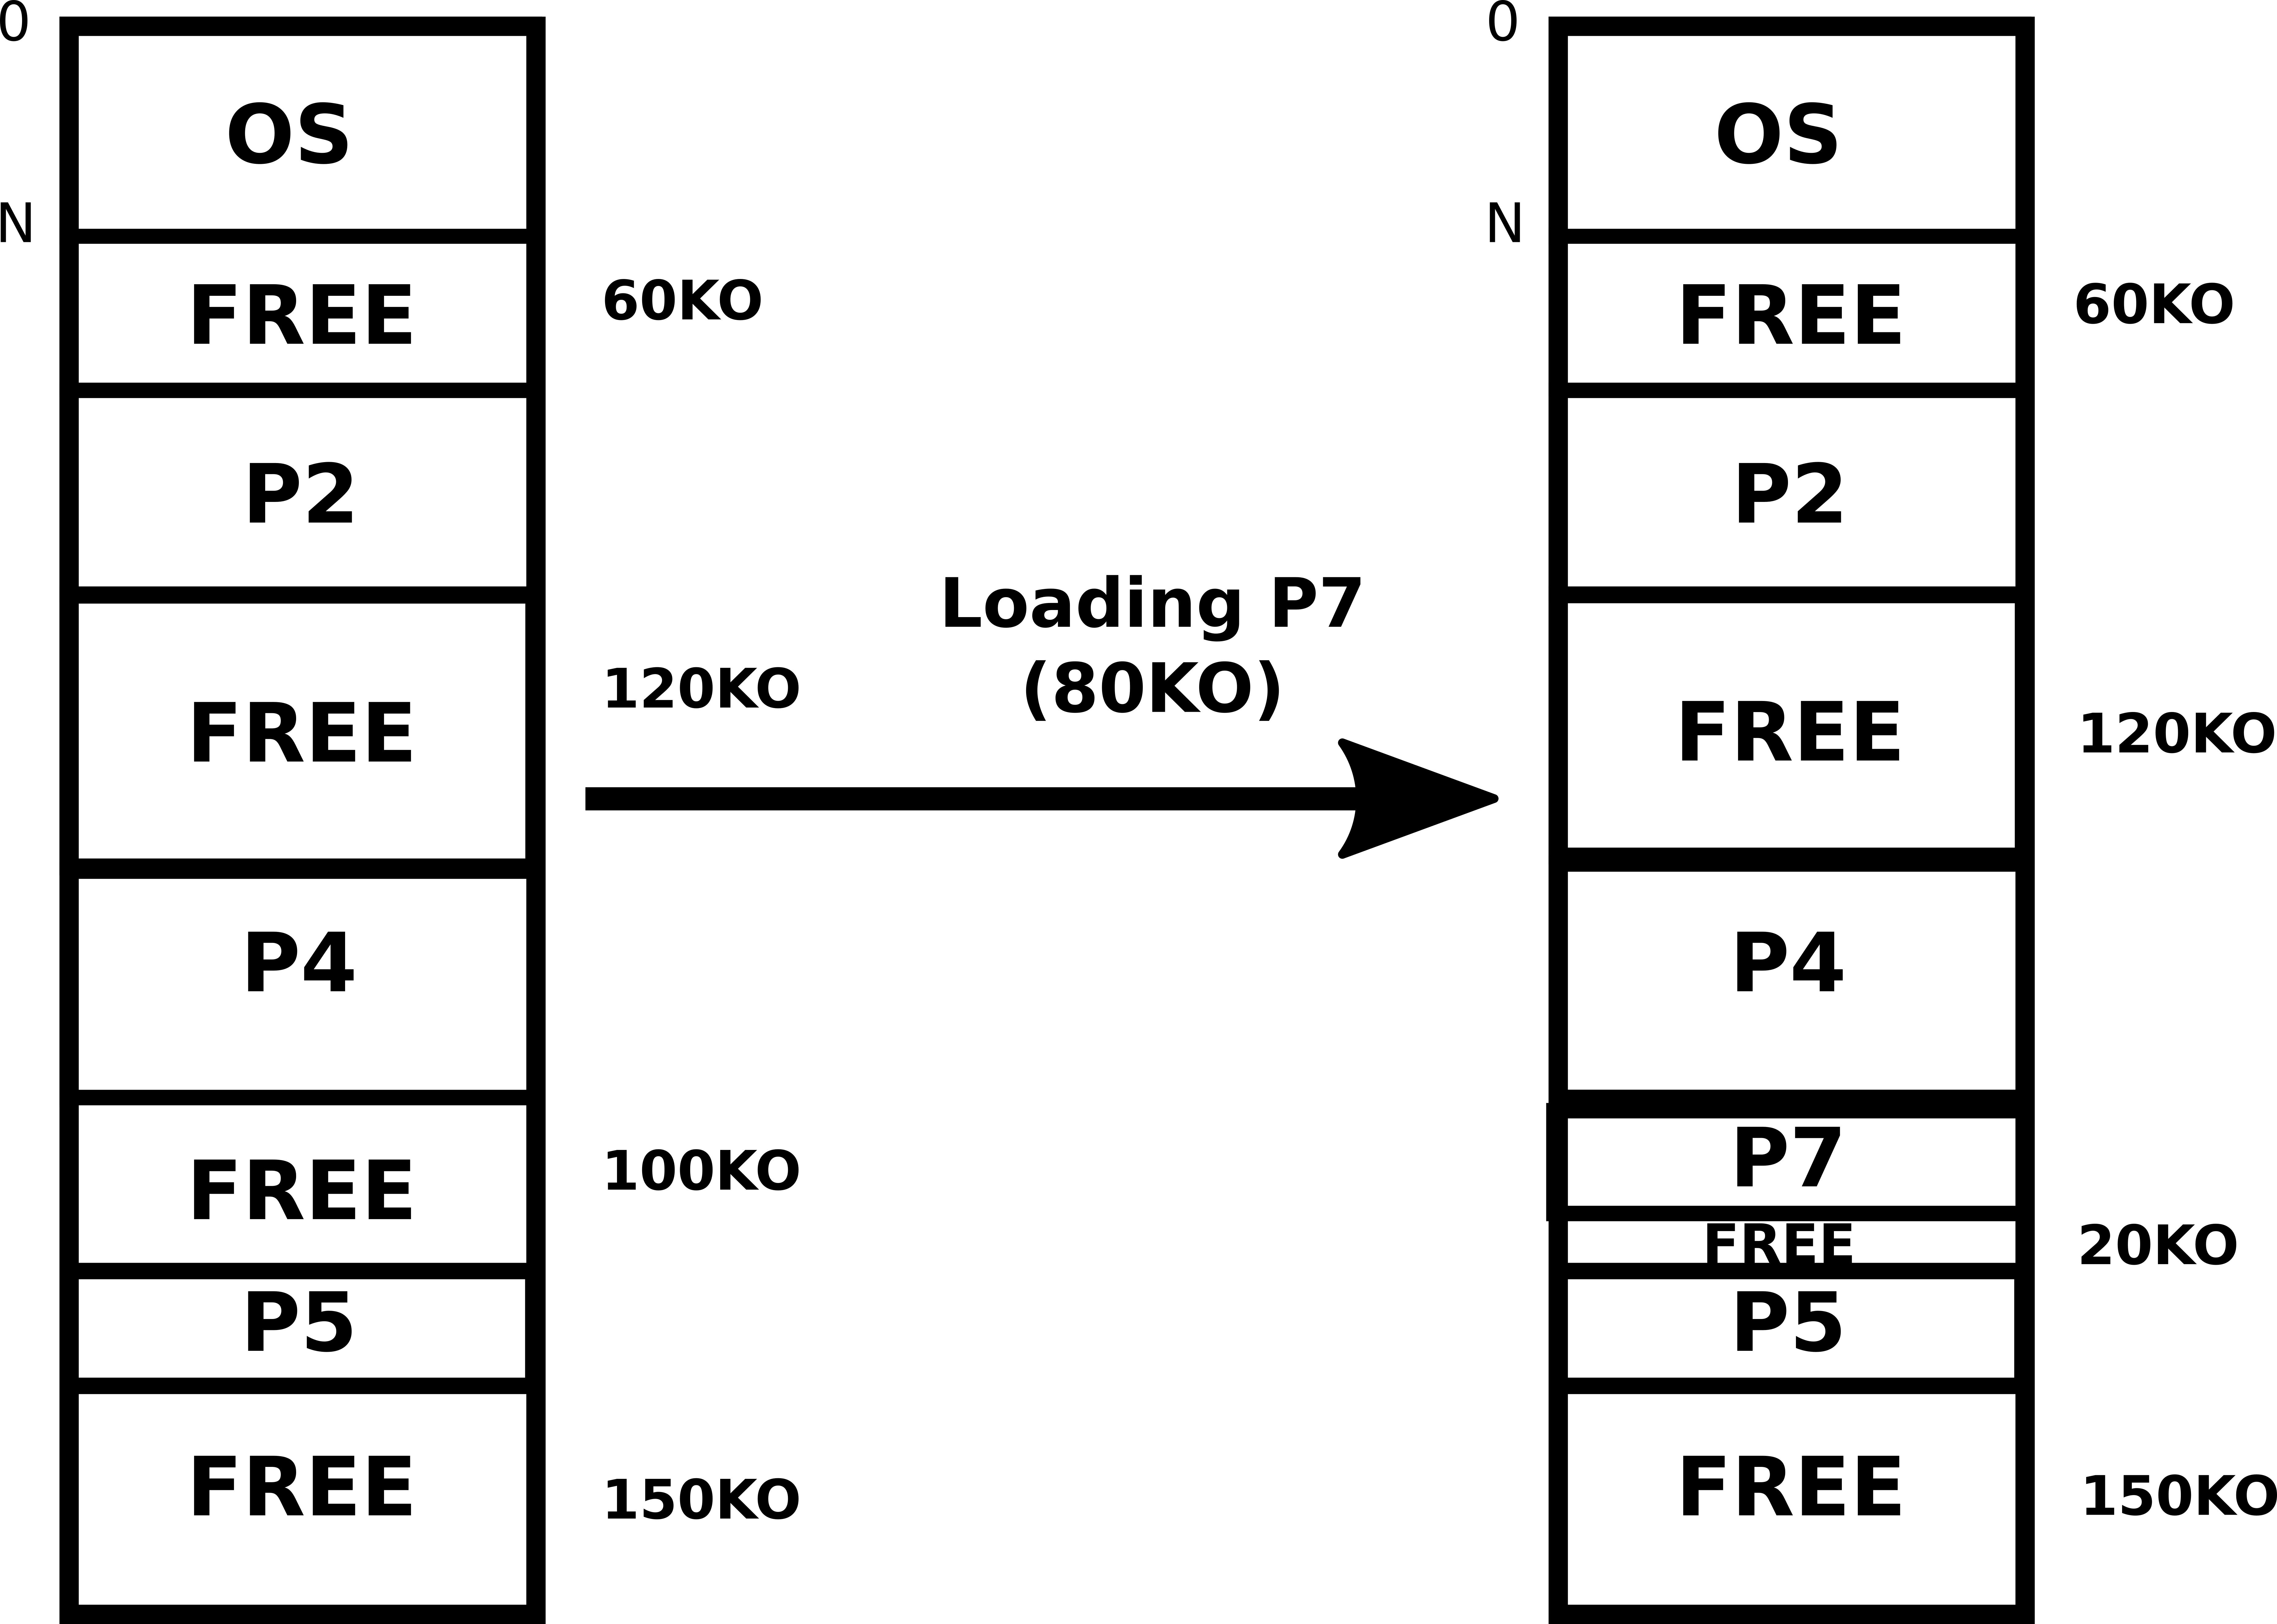
\includegraphics[scale=0.05]{images/p_mem_3.png} 
     	%\vspace*{-0.5em}
		%\caption{Floating gate transistor cell}
	\end{figure}			
	
	\vspace*{1em}	
	\begin{itemize}
	\item{Advantage: \textbf{best main memory usage} (20KO)}
	\item{BUT: \textbf{slow} (need to examine the memory to have the best fitting area)}
	\end{itemize}		
	
	\end{frame}	    	
	    	
	\begin{frame}
	
	The "\textit{Worst free area}" strategy:
	\vspace*{1em}
	\begin{figure}
		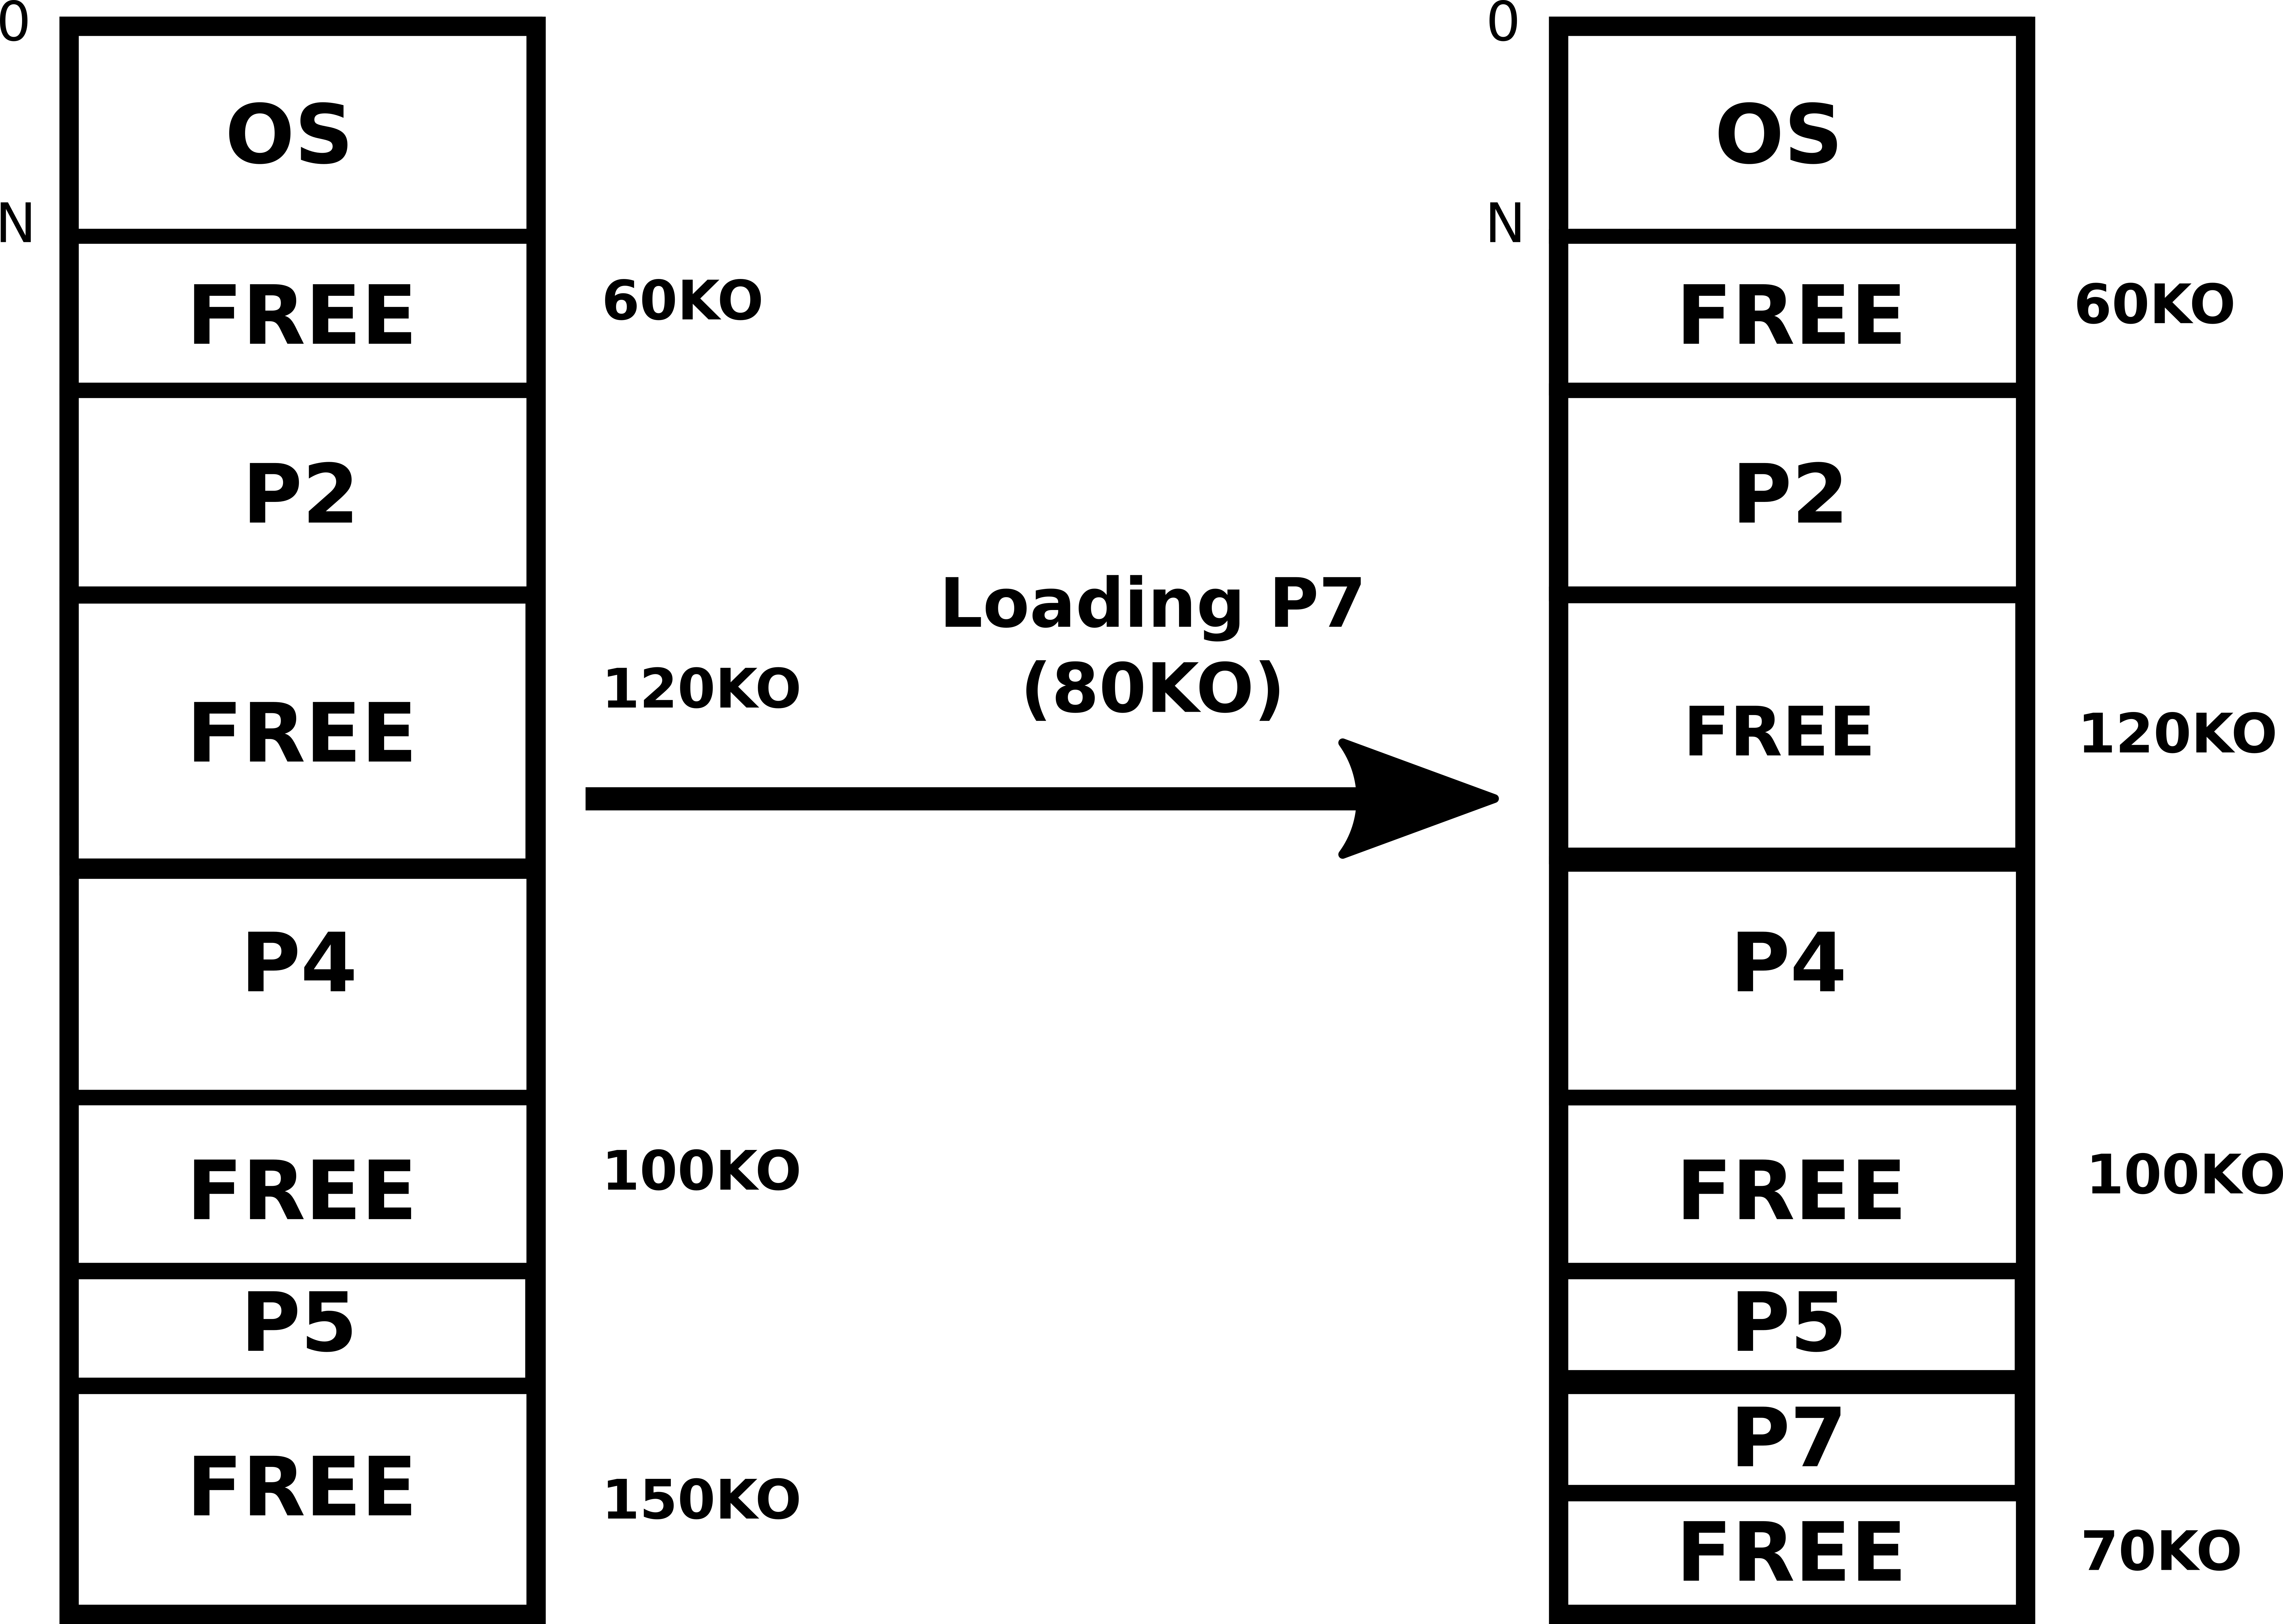
\includegraphics[scale=0.05]{images/p_mem_4.png} 
     	%\vspace*{-0.5em}
		%\caption{Floating gate transistor cell}
	\end{figure}
	
	\vspace*{1em}
	\begin{itemize}
	\item{Advantage: create \textbf{bigger memory fragments} (can be used after!)}
	\item{BUT: \textbf{slow} (need to examine the memory to have the best fitting area)}
	\end{itemize}
	
	\end{frame}	    	
	
	\subsection{Fragmentation}	
	
	\begin{frame}
	\begin{block}{Fragmentation?}
	Memory gets \textit{fragmented} rapidly:
	\begin{itemize}
	\item{Process \textbf{creations and terminations} fragment the memory}
	\item{When too fragmented the memory \textbf{may become unusable}!}
	\end{itemize}
	\end{block}
	
	\begin{figure}
		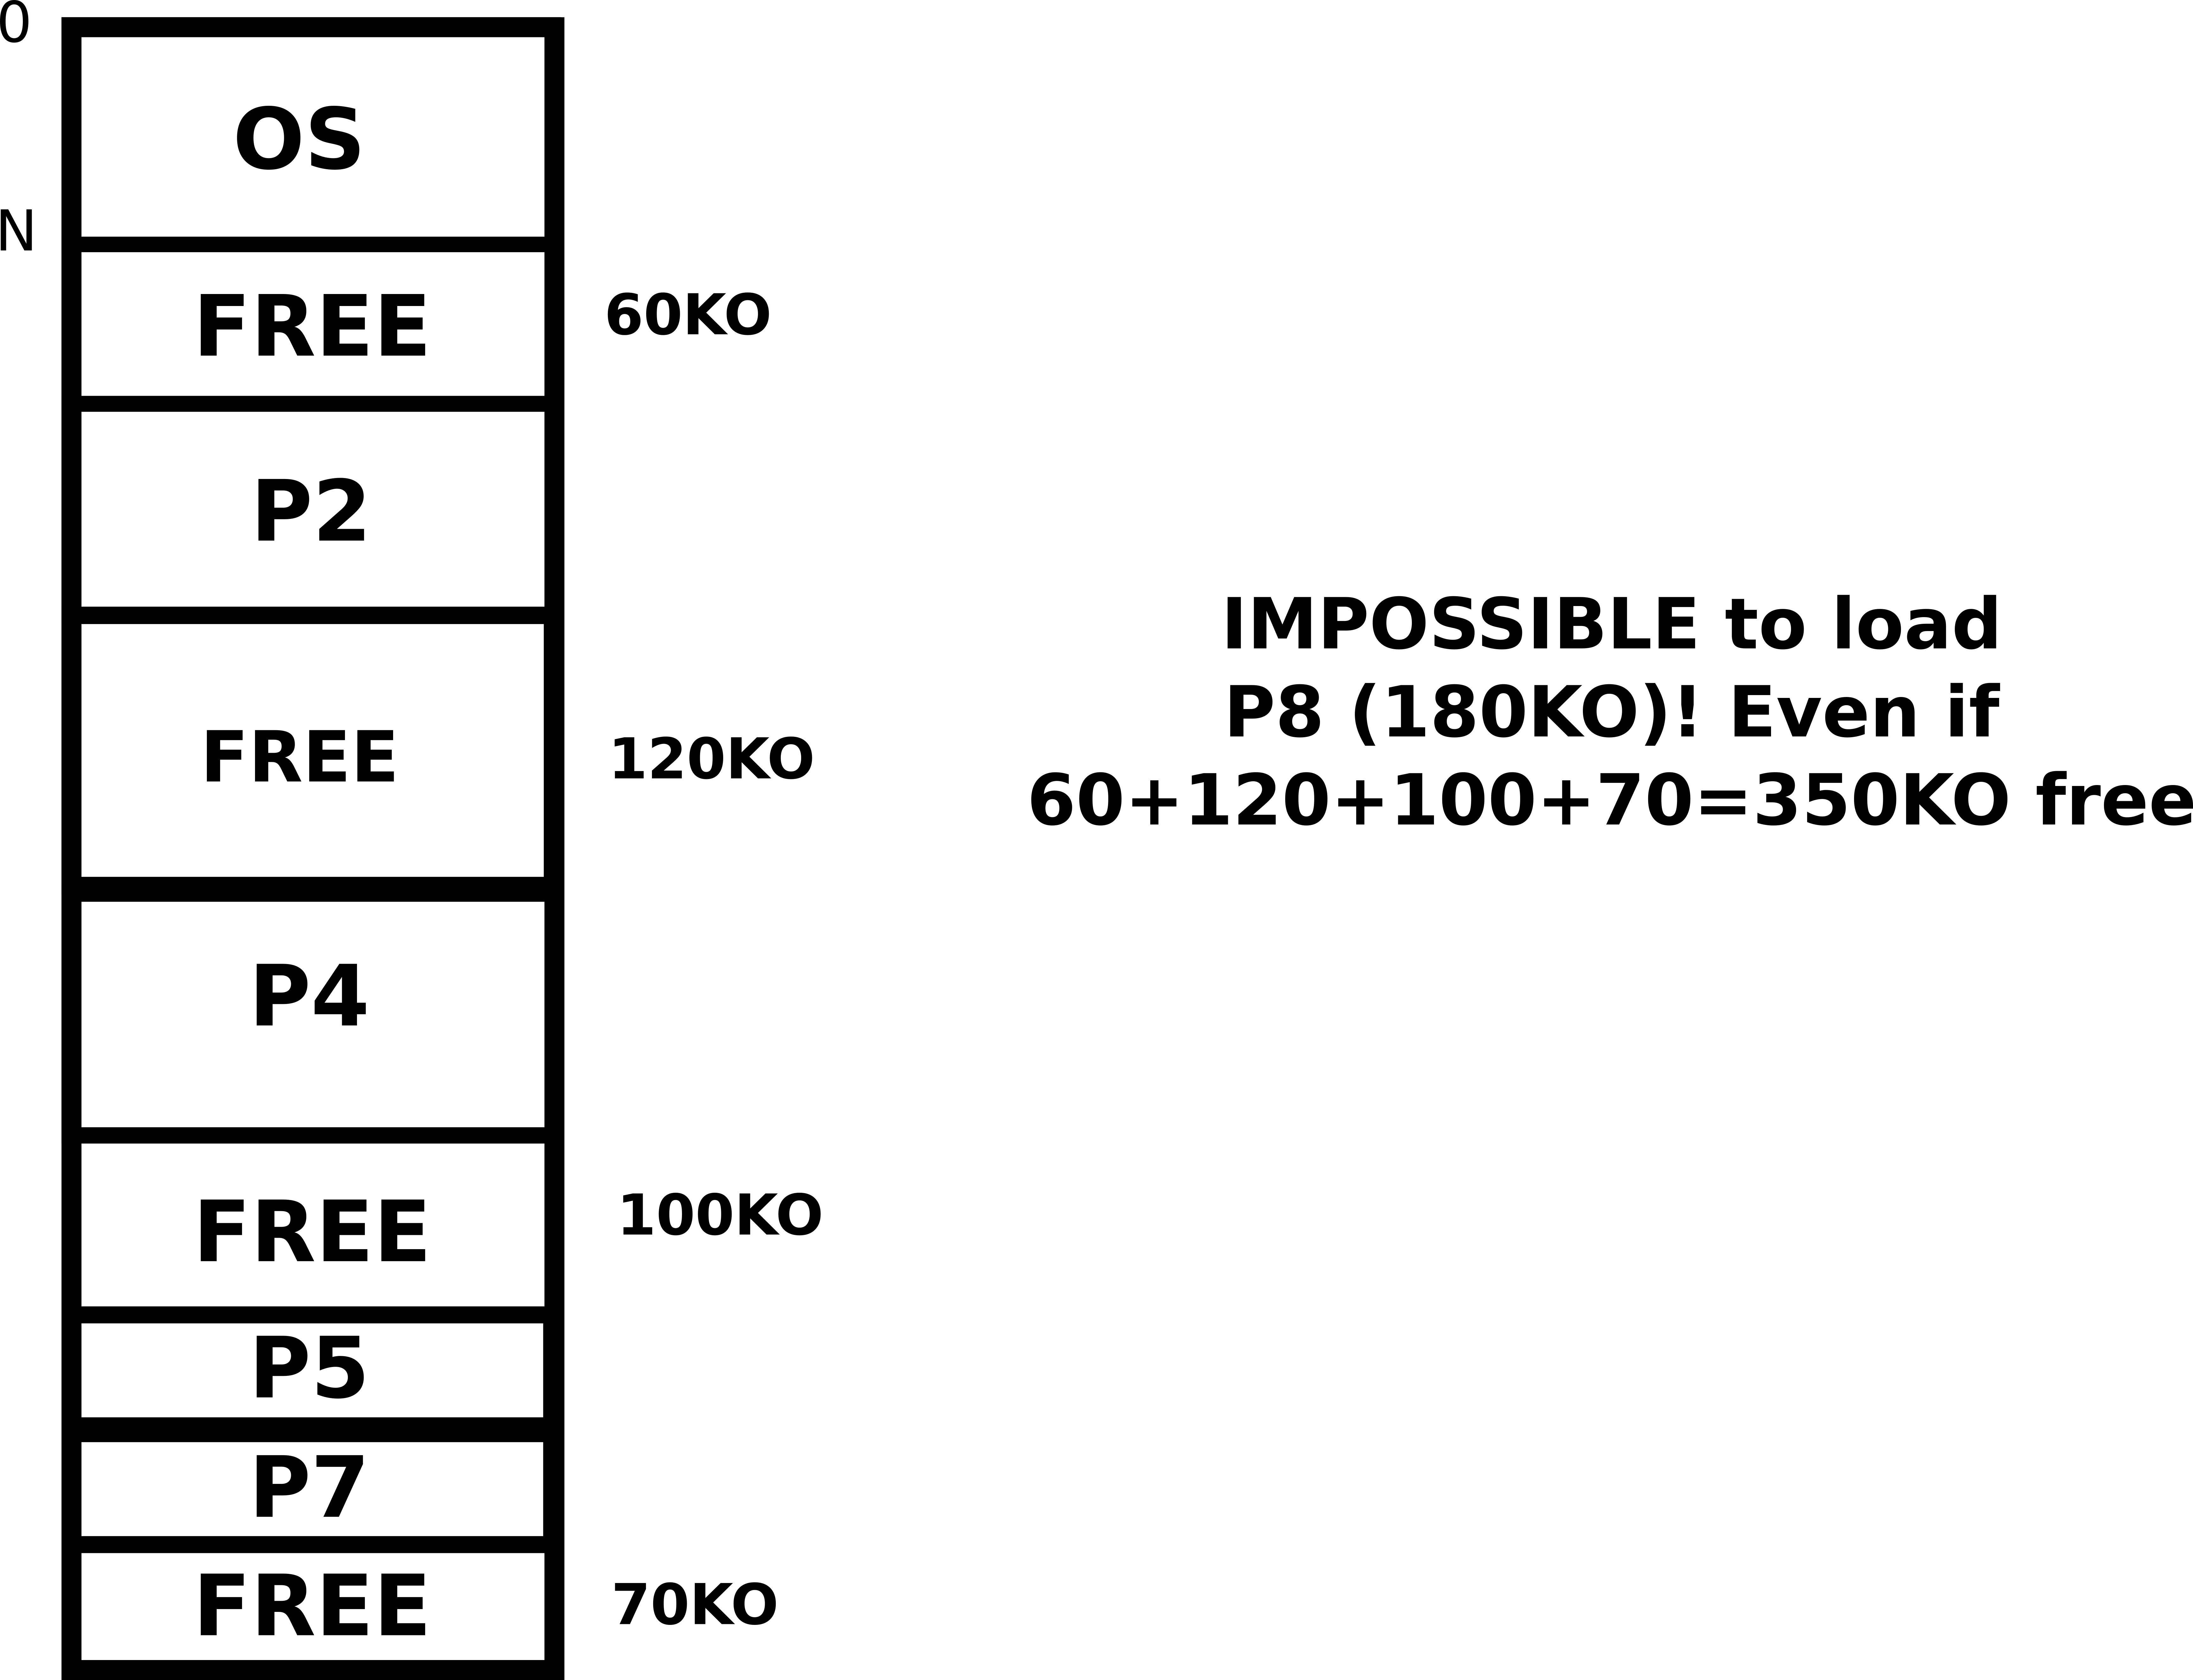
\includegraphics[scale=0.05]{images/p_mem_5.png} 
     	%\vspace*{-0.5em}
		%\caption{Floating gate transistor cell}
	\end{figure}
	
	
	\end{frame}	    	
	
	\begin{frame}

	One solution is to \textbf{compact} the \textit{physical memory} first:
	
	\begin{figure}
		\includegraphics[scale=0.05]{images/p_mem_6.png} 
     	%\vspace*{-0.5em}
		%\caption{Floating gate transistor cell}
	\end{figure}		
	
	BUT: it is an \textbf{extremely slow} and \textbf{not optimized} approach	
	
	\end{frame}	

	\section{Non-contiguous memory allocation}
	\subsection{pagination}	
	
	\begin{frame}
	\begin{block}{Non-contiguous?}
	Here we consider that one \textit{program} = \textbf{several parts}
	\end{block}
	\vspace*{0.5em}
	Here ...:
	\vspace*{1em}
	\begin{itemize}
	\item{each part has an \textbf{equal size} and is called: a \textbf{page}}
	\item{the parts \textbf{can be at very different locations} in main memory}
	\item{the \textit{physical memory} is divided in \textbf{empty cases of equal sizes} (512 to 8192 bytes)}
	\end{itemize}		
	\vspace*{1em}	
	We call this memory allocation mechanism: the \textbf{pagination}
	\end{frame}

	\subsection{Conversion of paginated addresses into physical addresses}	    
	\begin{frame}
	
	Because the \textit{physical memory} is divided in pages the memory is ...
	\vspace*{1em}
	\begin{itemize}
	\item{... accessed giving a page index \textit{p} and a displacement \textit{d} inside it
	\begin{itemize}
	\item{example: <p,d>}
	\end{itemize} }
	\end{itemize}	
	
	\begin{figure}
		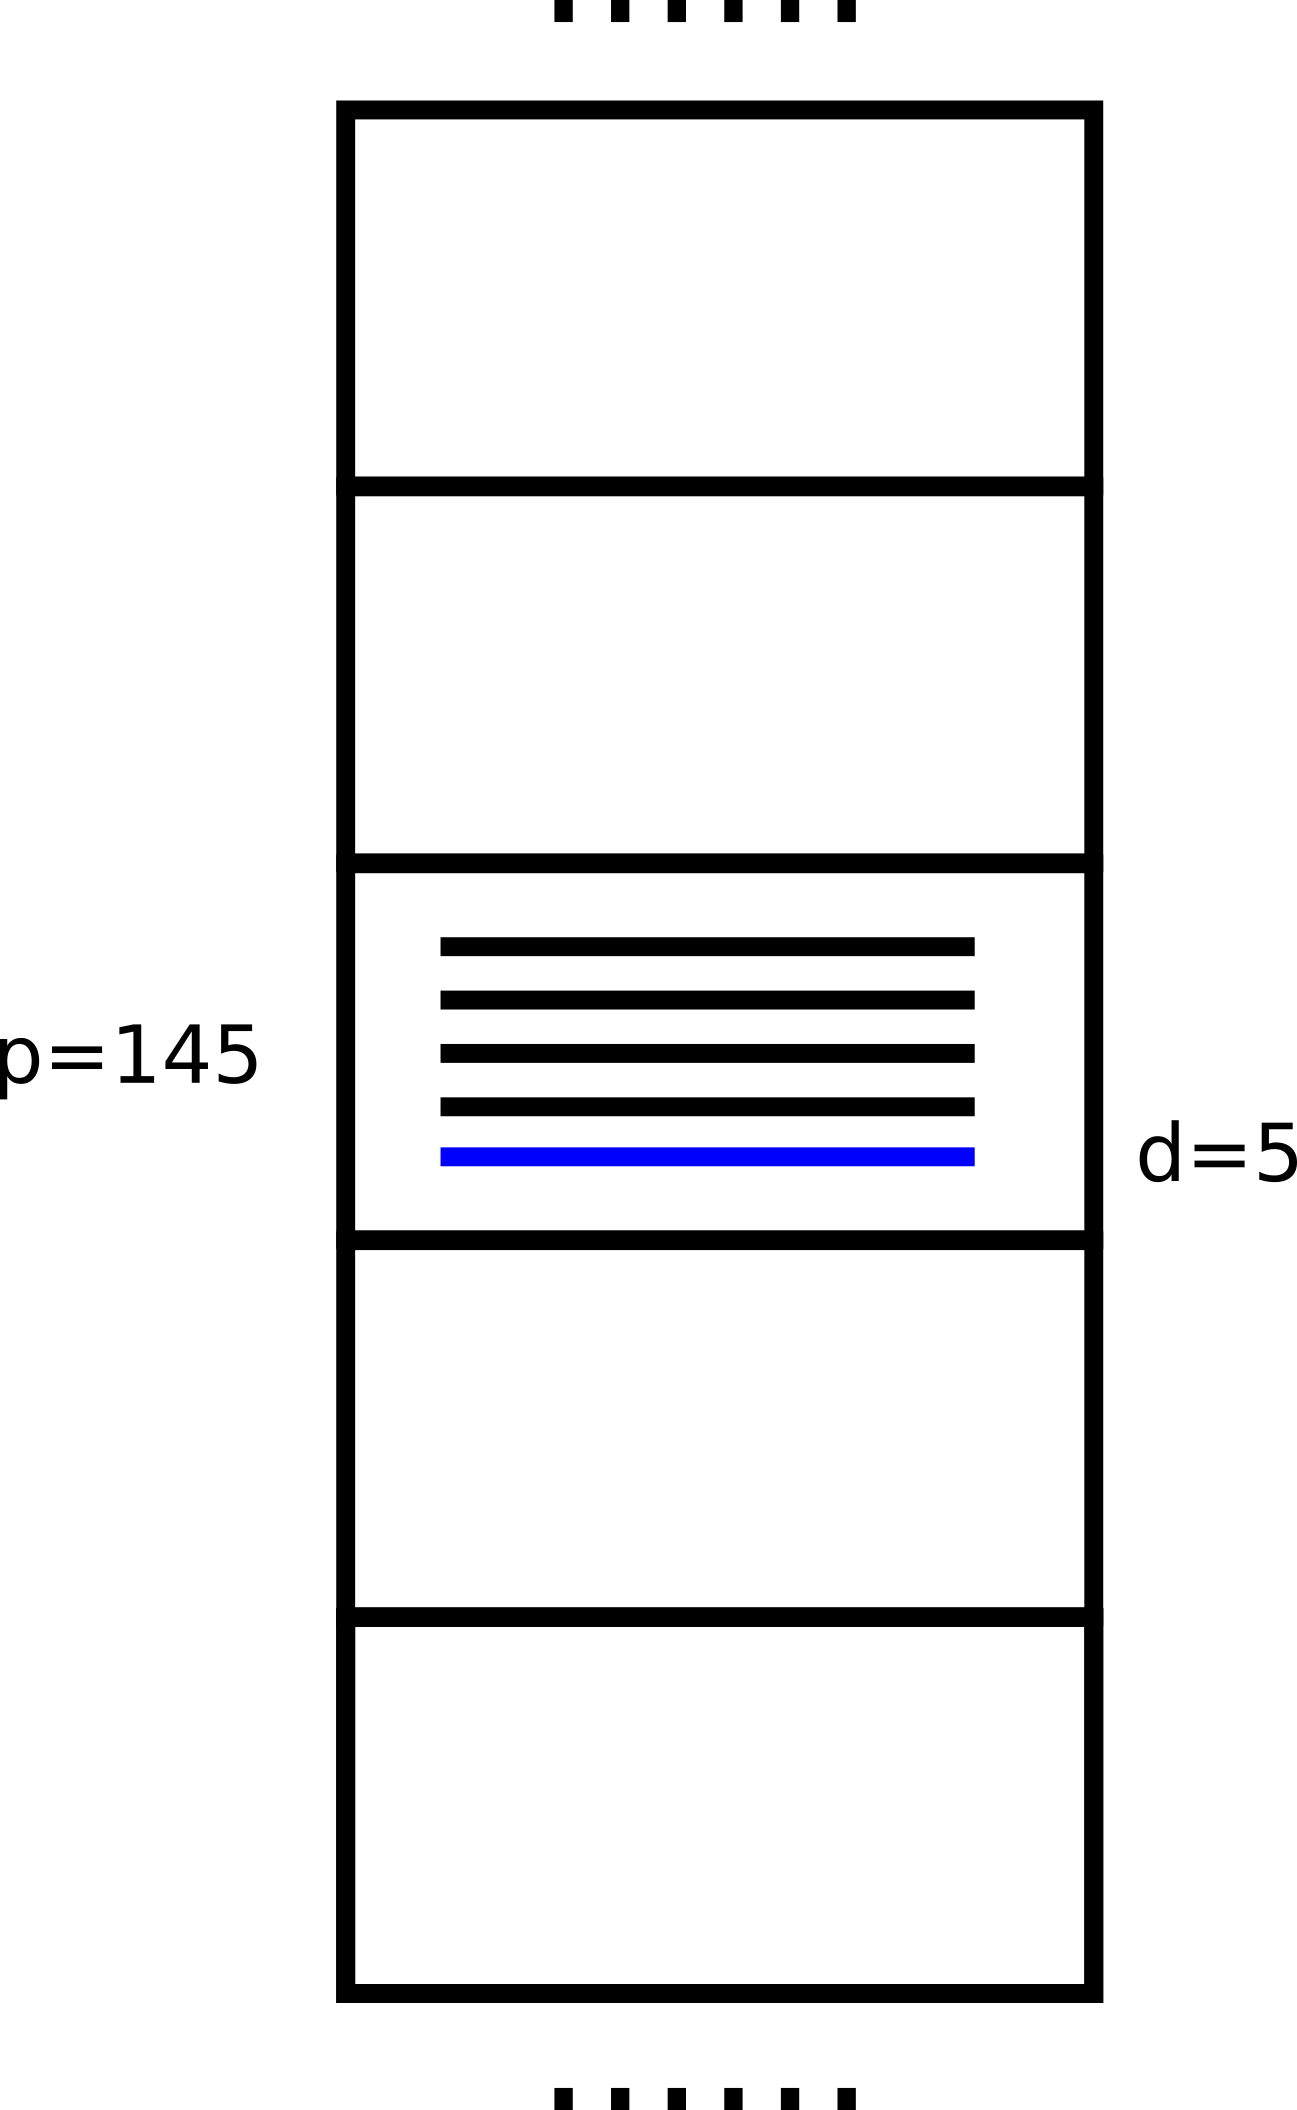
\includegraphics[scale=0.1]{images/pages_1.png} 
     	%\vspace*{-0.5em}
		%\caption{Floating gate transistor cell}
	\end{figure}		
	
	\begin{block}{Note}
	\textit{paginated addresses} are converted to \textit{physical addresses} later (for CPU)
	\end{block}		
	
	\end{frame}   	
	
	\subsection{Pagination in details}	
	
	\begin{frame}
		
	\begin{figure}
		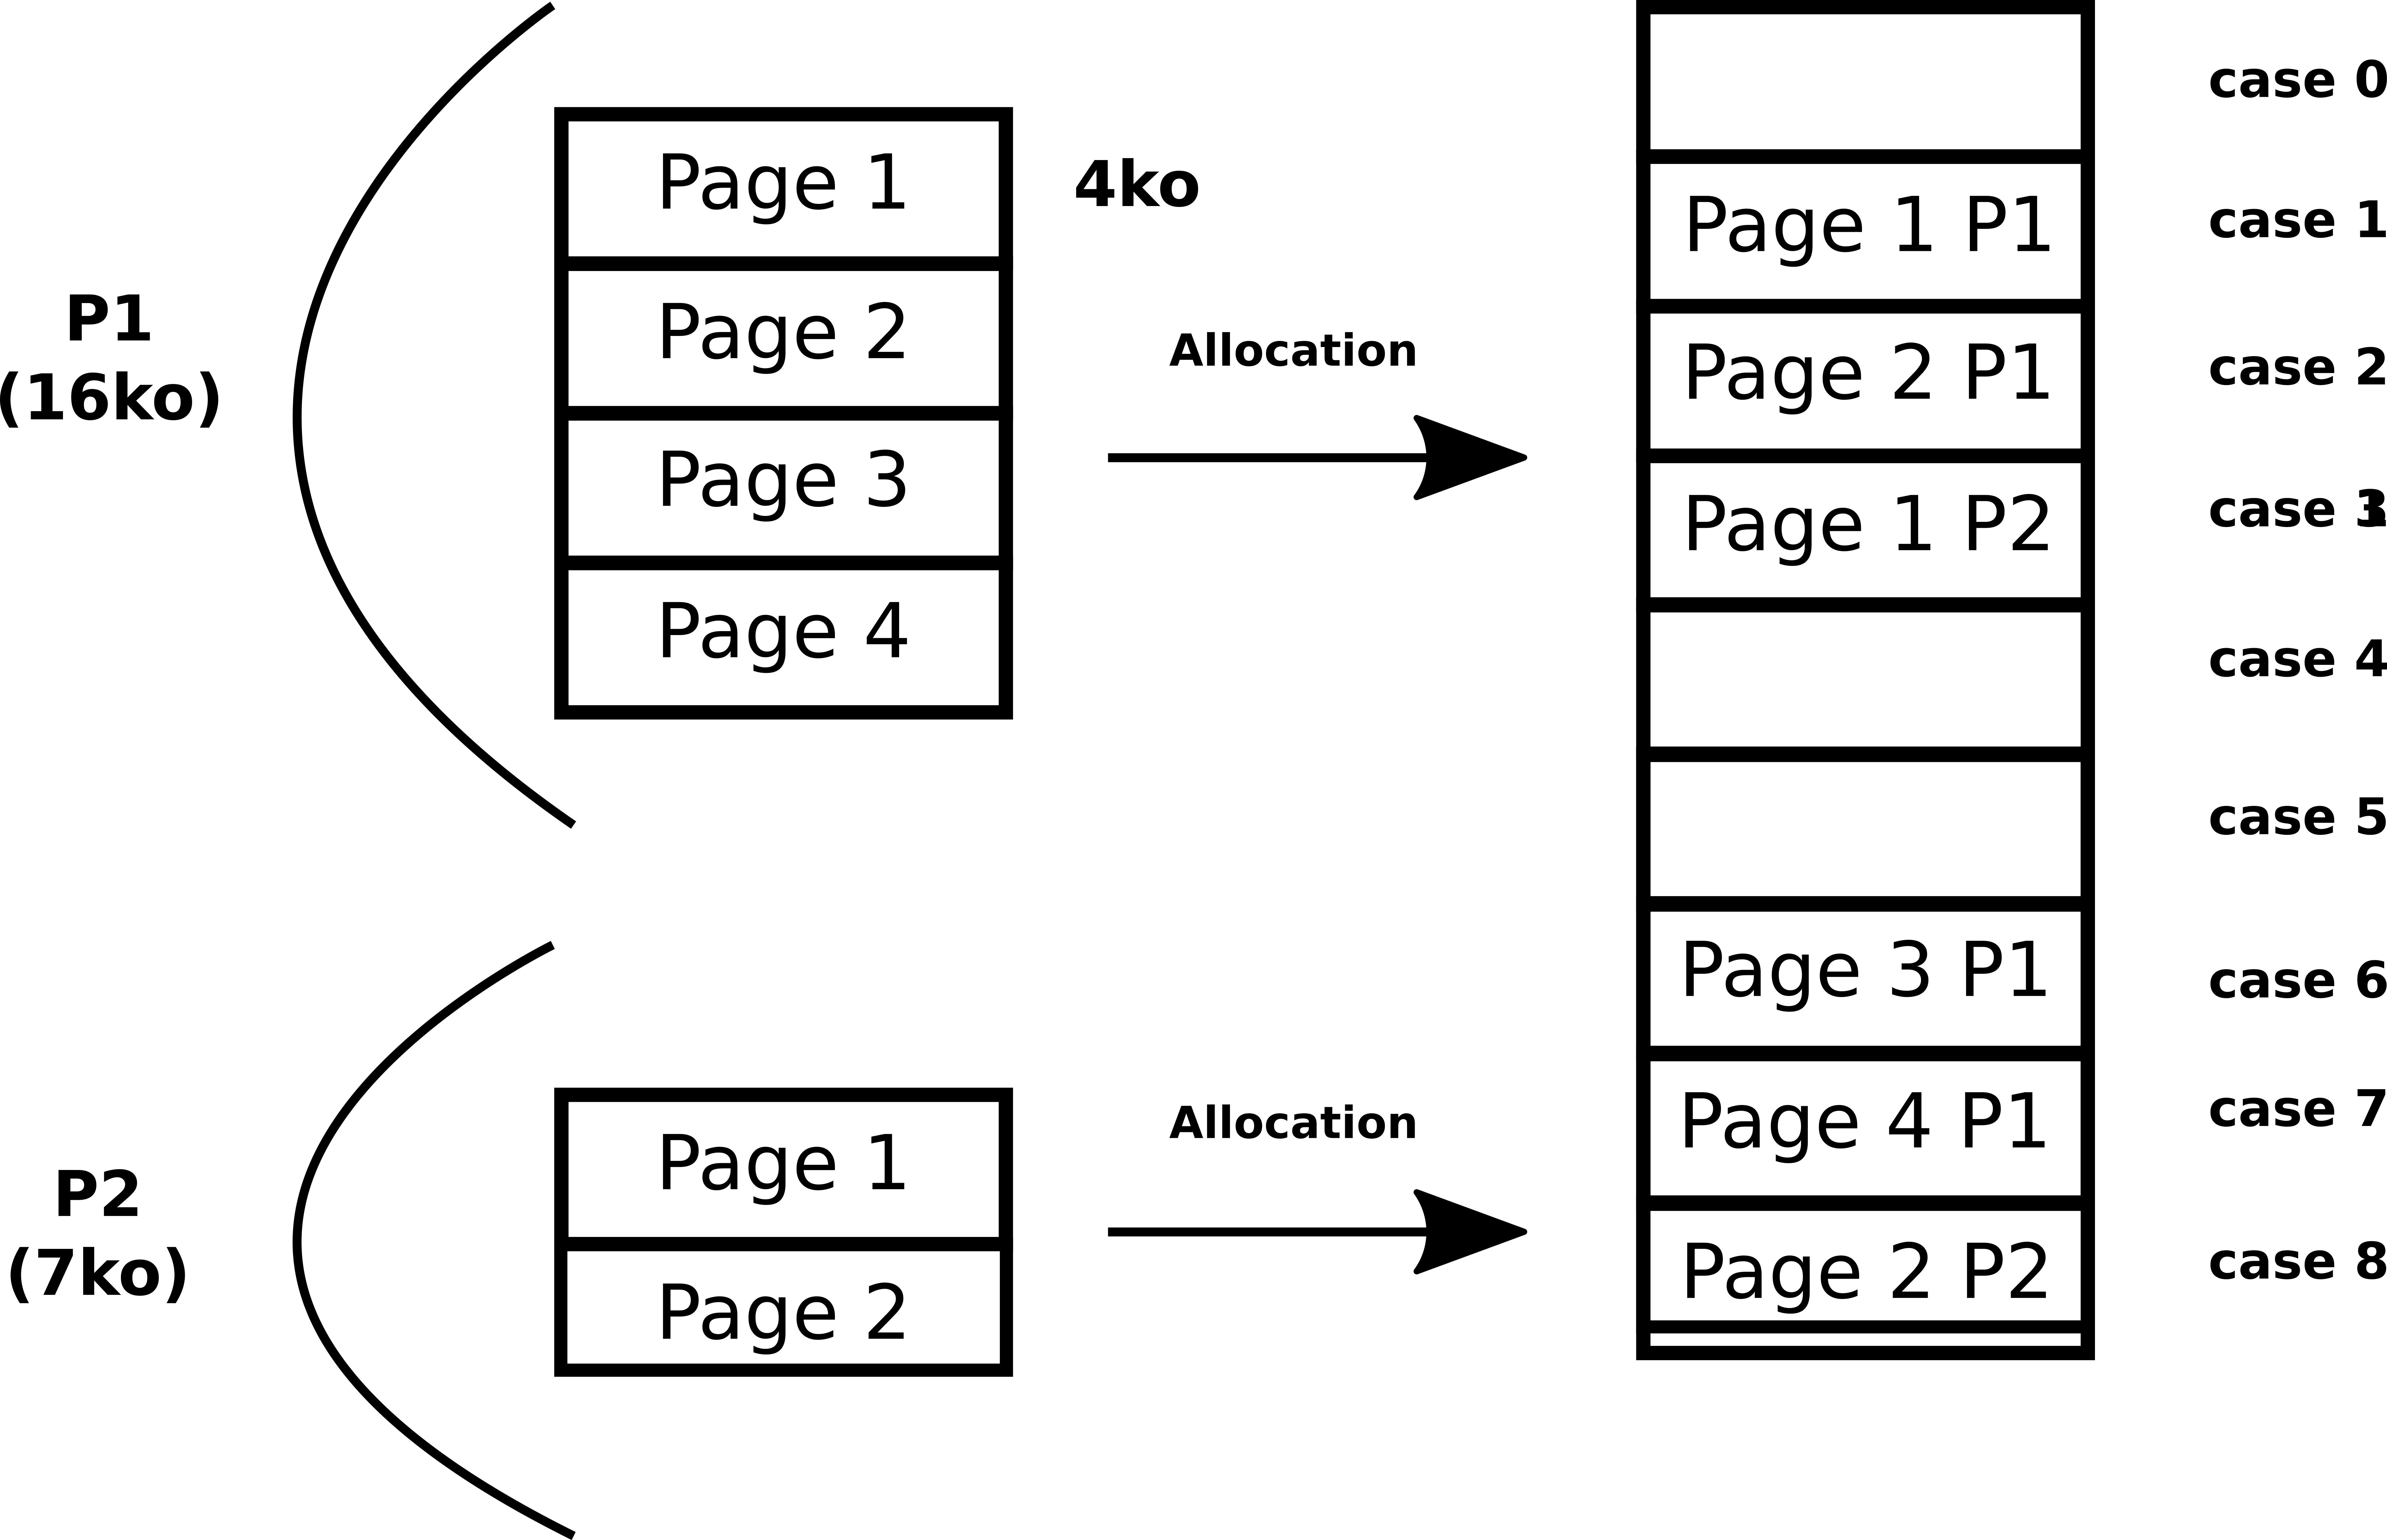
\includegraphics[scale=0.07]{images/pages_2.png} 
     	%\vspace*{-0.5em}
		%\caption{Floating gate transistor cell}
	\end{figure}	
	
	\begin{block}{Note}
	With \textit{pagination} the \textit{memory fragmentation} is not a problem!
	\end{block}	
	
	
	\end{frame}
	
	\begin{frame}
	
	To know where are all program pages we haves: the \textit{table of pages}.
	Example:
	\vspace*{1em}
	
	\begin{center}
	\begin{tabular}{|c|c|c|}
	\hline
	case & page & program \\ \hline
	0 & -1 & \\ \hline
	1 & 1 & P1 \\ \hline
	2 & 2 & P1 \\ \hline
	3 & 1 & P2 \\ \hline
	4 & -1 & \\ \hline
	5 & -1 & \\ \hline
	6 & 3 & P1 \\ \hline
	7 & 4 & P1 \\ \hline
	8 & 2 & P2 \\ \hline
	
	\end{tabular}	
	\end{center}
	
	\vspace*{1em}
	\begin{block}{Note}
	\textit{-1} in the \textit{table of pages} just mean that this case is not occupied by a page
	\end{block}	
		
	\end{frame}	
	
	\section{Virtual memory}
	\subsection{Introduction}	
	\begin{frame}
	
	It comes from an observation: \textbf{not all pages are always necessary}:
	\vspace*{1em} 	
	\begin{itemize}
	\item{Only \textbf{a small amount of a pages} need to be in physical memory}
	\item{The \textbf{rest can stay in mass storage} (in the virtual memory)}
	\end{itemize}
	\vspace*{1em}	
	Here our \textit{table of pages} has another column (V)\footnotemark[2]:
	
		\begin{center}
	\begin{tabular}{|c|c|c|c|}
	\hline
	case & page & program & V\\ \hline
	0 & -1 & & 0\\ \hline
	1 & 1 & P1 & 1\\ \hline
	-1 & 2 & P1 & 0\\ \hline
	-1 & 1 & P2 & 0\\ \hline
	4 & -1 & & 0\\ \hline
	5 & -1 & & 0\\ \hline
	6 & 3 & P1 & 1 \\ \hline
	-1 & 4 & P1 & 0 \\ \hline
	8 & 2 & P2 & 1\\ \hline
	
	\end{tabular}	
	\end{center}	
	
	
	\footnotetext[2]{When V=1: page in \textit{physical memory}, V=0: page in \textit{virtual memory}}
	
	\end{frame}
		
	\begin{frame}
	
		\begin{center}
	\begin{tabular}{|c|c|c|c|}
	\hline
	case & page & program & V\\ \hline
	0 & -1 & & 0\\ \hline
	1 & 1 & P1 & 1\\ \hline
	-1 & 2 & P1 & 0\\ \hline
	-1 & 1 & P2 & 0\\ \hline
	4 & -1 & & 0\\ \hline
	5 & -1 & & 0\\ \hline
	6 & 3 & P1 & 1 \\ \hline
	-1 & 4 & P1 & 0 \\ \hline
	8 & 2 & P2 & 1\\ \hline
	
	\end{tabular}	
	\end{center}	
	
	
	\vspace*{1em}	
	\begin{block}{Note}
	When we have V=0 for a page: the system \textbf{detects it in advance} and loads the page in main memory so that the \textit{CPU} can execute smoothly the instructions in the page, without stopping.
	\end{block}
	
	
	\end{frame}		
	
	\subsection{Percentage of pages per program}	
			
	\begin{frame}
	
	There are two approaches to attribute the number of cases per program:
	\vspace*{1em}
	\begin{enumerate}
	\item{Giving the same number of cases per program
	\begin{itemize}
	\item{BUT: a small process can have as many as a big process}
	\end{itemize}
	}
	\item{Giving a proportionate to the size number of cases
	\begin{itemize}
	\item{Advantage: bigger processes have more cases}
	\end{itemize}		
	}
	\end{enumerate}
		
	\vspace*{1em}		
		
	Indeed, processes in \textbf{main memory} may have very different sizes...	
	
	\vspace*{1em}
	
	\begin{block}{Note}
	A process has an initial \textbf{number of cases} used to load its active pages:
	\begin{itemize}
	\item{number of cases per program < total number of program pages}
	\end{itemize}
	\end{block}
	
	
	\end{frame}	
	
	\subsection{Replacing pages}	
	
	\begin{frame}
		
	When a \textit{process} has used all its available cases:
	\vspace*{1em}
	\begin{itemize}
	\item{a \textbf{new case must be found} for loading the next page!}
	\item{a case can be found by \textbf{replacing an existing page}!}
	\item{either in its \textbf{own initially attributed cases}}
	\item{or in \textbf{others' attributed cases}}
	\end{itemize}
	\vspace*{1em}
	\pause
	There are several algorithms to find the ideal \textit{victim page}:
	\vspace*{1em}
	\begin{itemize}
	\item{The \textit{FIFO} replacement algorithm}
	\item{The \textit{Least Recently Used} replacement algorithm}
	\item{The \textit{second chance} algorithm}
	\item{The \textit{Least Frequently Used} replacement algorithm}
	\item{The \textit{Most Frequently Used} replacement algorithm} 
	\end{itemize}		
		
	
	\end{frame}		
	
	\begin{frame}
	
	\begin{itemize}
	\item{The \textit{FIFO} replacement algorithm:
	\vspace*{1em}
	
	The oldest loaded page is replaced 	
	\vspace*{1em}
	}
	\item{The \textit{Least Recently Used} replacement algorithm:
	\vspace*{1em}	
	
	The least used page is replaced. This algorithm is one of the most used. But, it is hard to implement and require extra hardware.
	\vspace*{1em}	
	}
	\item{The \textit{second chance} algorithm:
	\vspace*{1em}
	
	This algorithm is an approximation of the LRU algorithm. Less complex to implement.
	\vspace*{1em}	
	}
	\end{itemize}		
	
	\end{frame}
	
	\begin{frame}
	
	\begin{itemize}
	\item{The \textit{Least Frequently Used} replacement algorithm:
	\vspace*{1em}
	
	The least frequently used page is replaced. But it raises problems when a large number of pages are loaded in a short time: they risk to be replaced first!	
	\vspace*{1em}
	}
	\item{The \textit{Most Frequently Used} replacement algorithm
	\vspace*{1em}	
	
	Here, the most frequently used page is replaced. There is an opposite logic here: we consider that a page that is not used a lot needs to stay in memory.
	\vspace*{1em}	
	}
	\end{itemize}		
	
	\end{frame}
	
		
	
	
\end{document}
